
\chapter{INTRODUCTION}

\section{Privacy Systems}

% privacy - breaking the link
% anonymity - cannot be identified, communiciations are indistinguishable from other messages, untrackable, part of privacy
% confidentiality - protecting the secret, VPNs claim to give anonymity by holding identities in confidence
% 

As the prevalence of the Internet and other communication has grown, so too has the development and usage of privacy-enhancing systems. These are tools and protocols that provide privacy by obfuscating the link between a user's identification or location and their communications. A closely related property is anonymity -- a part of privacy where user activities cannot be tracked and their communications are indistinguishable from others. Tools that provide these systems hold a user's identity in confidence, and privacy and anonymity are often provided together. Following a general distrust of unsecured Internet communications and in light of the 2013-current revelations by Edward Snowden of Internet surveillance by the Five Eyes, users have increasingly turned to these tools for their own protection. Privacy-enhancing and anonymity tools may also be used by the military, researchers working in sensitive topics, journalists, law enforcement running tip lines, activists and whistleblowers, or individuals in countries with Internet censorship. These users may turn to proxies or VPNs, but these tools rarely provide anonymity and they can easily break confidence to destroy user privacy. More complex tools are needed for a stronger guarantee of privacy and anonymity.

Today, most anonymity tools descent from mixnets, a concept invented by David Chaum in 1981.\cite{chaum2003untraceable} In a mixnet, user messages are transmitted to one or more mixes, who each partially decrypt, scramble, delay, and retransmit the messages to other mixes or to the final destination. This enhances privacy by heavily obscuring the correlation between the origin, destination, and contents of the messages. Mixnets have inspired the development of many varied mixnet-like protocols and have generated significant literature within the field of network security.\cite{edman2009anonymity}\cite{syverson2011peel}

Mixnet descendants can generally be classified into two distinct categories: high-latency and low-latency systems. High-latency networks typically delay traffic packets and are notable for their greater resistance to global adversaries who monitor communication entering and exiting the network. However, high-latency networks, due to their slow speed, are typically not suitable for common Internet activities such as web browsing, instant messaging, or the prompt transmission of email. Low-latency networks, by contrast, do not delay packets and are thus more suited for these activities, but they are more vulnerable to timing attacks from global adversaries.\cite{dingledine2004tor} In this work, we detail and introduce new functionality within low-latency protocols.

Onion routing is a technique for enhancing privacy of TCP-based communication across a network and is the most popular low-latency descendant of mixnets in use today. It was first designed by the U.S. Naval Research Laboratory in 1997 for military usage \cite{syverson1997anonymous}\cite{reed1998anonymous} but has since seen widespread usage. In onion routing with public key infrastructure (PKI), a user selects a set network nodes, typically called \emph{routers}, and encrypts the message with the public key of each router. Each encryption layer contains the next destination for the message -- the last layer contains the message's final destination. As the message travels through the network, each of these routers in turn decrypt their encryption layer like an onion, exposing their share of the routing information. The final recipient receives the message from the last router, but is never exposed to the message's source.\cite{syverson2011peel} 

\begin{figure}[htbp]
	\centering
	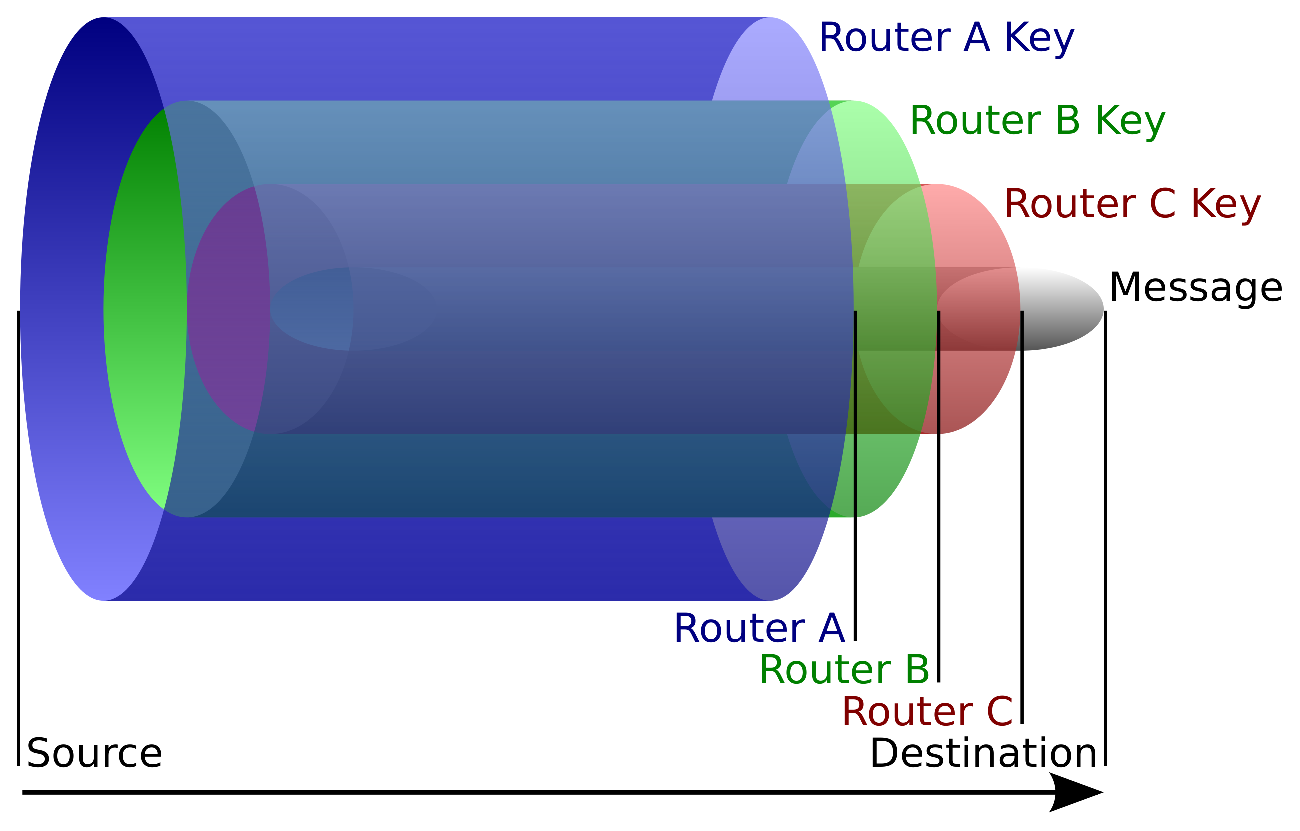
\includegraphics[width=0.5\textwidth]{images/onion-diagram.eps}
	\caption{Example of message encryption in an onion routing scheme. Each router ``peals'' off its respective layer of encryption; the final router exposes the final destination.}
\end{figure}

Onion routing can also utilize symmetric-key cryptography for increased efficiency and perfect-forward secrecy. In this system, a user Alice initializes the series of routers (known as a \emph{circuit}) by negotiating a Diffie-Hellman-Merkle ephemeral key exchange with each of the routers in turn, extending the circuit one node at a time. Alice's messages to Bob and intermediate routing information is then encrypted with each of these keys in turn. If routers remember the destinations for each message they received, Bob can send his reply backwards through the circuit and each router re-encrypts the reply with their ephemeral symmetric key. Alice unwraps all the layers, exposing the Bob's reply. This system facilitates low-latency privacy-enhanced communication because at no point are packets delayed and symmetric cryptography is significantly less computationally intensive than asymmetric public key cryptography. Alice has privacy because Bob does not know her location and she has anonymity if she does not include any identification or distinguishing information in her message.\cite{syverson2011peel}\cite{dingledine2004tor}

\section{Tor}




The Tor network is a second-generation onion routing system that aims to provide anonymity, privacy, and Internet censorship protection to its users. The Tor client software multiplexes all end-user TCP traffic through a series of relays on the Tor network, typically a carefully-constructed three-hop path known as a \textit{circuit}. Each relay in the circuit has its own encryption layer, so traffic is encrypted multiple times and then is decrypted in an onion-like fashion as it travels through the Tor circuit. As each relay sees no more than one hop in the circuit, in theory neither an eavesdropper nor a compromised relay can link the connection's source, destination, and content. Tor remains one of the most popular and secure tools to use against network surveillance, traffic analysis, and information censorship.

While the majority of Tor's usage is for traditional access to the Internet, Tor's routing scheme also supports anonymous websites, hidden inside Tor. Unlike the Clearnet, Tor does not contain a traditional DNS system for its websites; instead, hidden services are identified by their public key and can be accessed through Tor circuits. A client and the hidden service can thus communicate anonymously.

The Tor network is a third-generation onion routing system, originally designed by the U.S. Naval Research Laboratory for protecting sensitive government communication. Tor refers both to the client-side multiplexing software and to the worldwide volunteer-run network of over six thousand nodes. The Tor software provides an anonymity and privacy layer to end-users by relaying TCP traffic through a series of relays on the Tor network. Tor sees global widespread use and as of January 2015 has over 2.4 million daily users and passes an average of approximately 6000 MB per second through its network.\cite{TorMetrics} Tor's encryption and routing protocols are designed to make it very difficult for an adversary to correlate an end user to their traffic. Tor has been recognized by the NSA as the "the king of high secure, low latency Internet anonymity".\cite{TorSlidesNSA}

\subsection{Design}

Tor routes encrypted TCP/IP user traffic through a worldwide volunteer-run network of over six thousand relays. Typically this route consists of a carefully-constructed three-hop path known as a \textit{circuit}, which changes over time. These nodes in the circuit are commonly referred to as \textit{guard node}, \textit{middle relay}, and the \textit{exit node}, respectively. Only the first node is exposed to the origin of TCP traffic into Tor, and only the exit node can see the destination of traffic out of Tor. The middle router, which passes encrypted traffic between the two, is unaware of either. The client negotiates a separate TLS connection with each node at a time, and traffic through the circuit is decrypted one layer at a time. As such, each node is only aware of the machines it talks to, and only the client knows the identity of all three nodes used in its circuit, making traffic correlation much more difficult difficult compared to a VPN, proxy, or a direct TLS connection.

The Tor network is maintained by nine authority nodes, who each vote on the status of nodes and together hourly publish a digitally signed consensus document containing IPs, ports, public keys, latest status, and capabilities of all nodes in the network. The document is then redistributed by other Tor nodes to clients, enabling access to the network. The document also allows clients to authenticate Tor nodes when constructing circuits, as well as allowing Tor nodes to authenticate one another. Since all parties have prior knowledge of the public keys of the authority nodes, the consensus document cannot be forged or modified without disrupting the digital signature.\cite{xin2009design}

\subsection{Routing}

In traditional Internet connections, the client communicates directly with the server. TLS encryption cannot hide IP and TCP headers, which must be exposed to allow routing. Eeavesdroppers can track end-users by monitoring these headers, easily correlating clients to their activities. Tor combats this by routing end user traffic through a randomized circuit through the network of relays. The client software first queries an authority node or a known relay for the latest consensus document. Next, the Tor client chooses three unique and geographically diverse nodes to use. It then builds and extends the circuit one node at at time, negotiating respective TLS connections with each node in turn. No single relay knows the complete path, and each relay can only decrypt its layer of decryption. In this way, data is encrypted multiple times and then is decrypted in an onion-like fashion as it passes through the circuit.

\begin{figure}[htdp]
	\begin{minipage}[b]{0.45\linewidth}
		\centering
		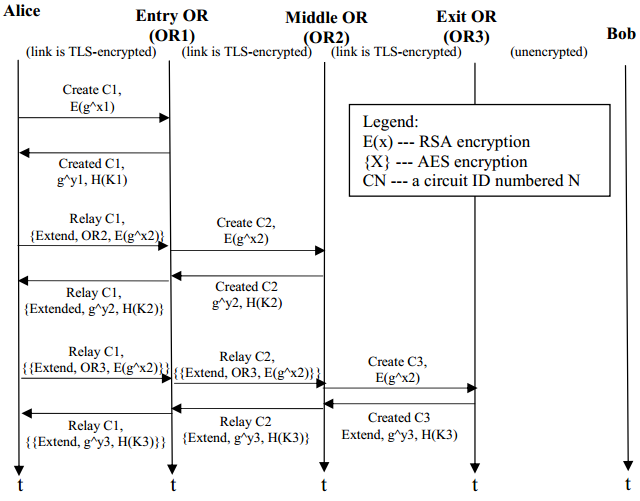
\includegraphics[width=\textwidth]{images/Tor/circuit-construction.png}
		\caption{Anatomy of the construction of a Tor circuit.}
		\label{fig:figure1}
	\end{minipage}
	\hspace{0.5cm}
	\begin{minipage}[b]{0.45\linewidth}
		\centering
		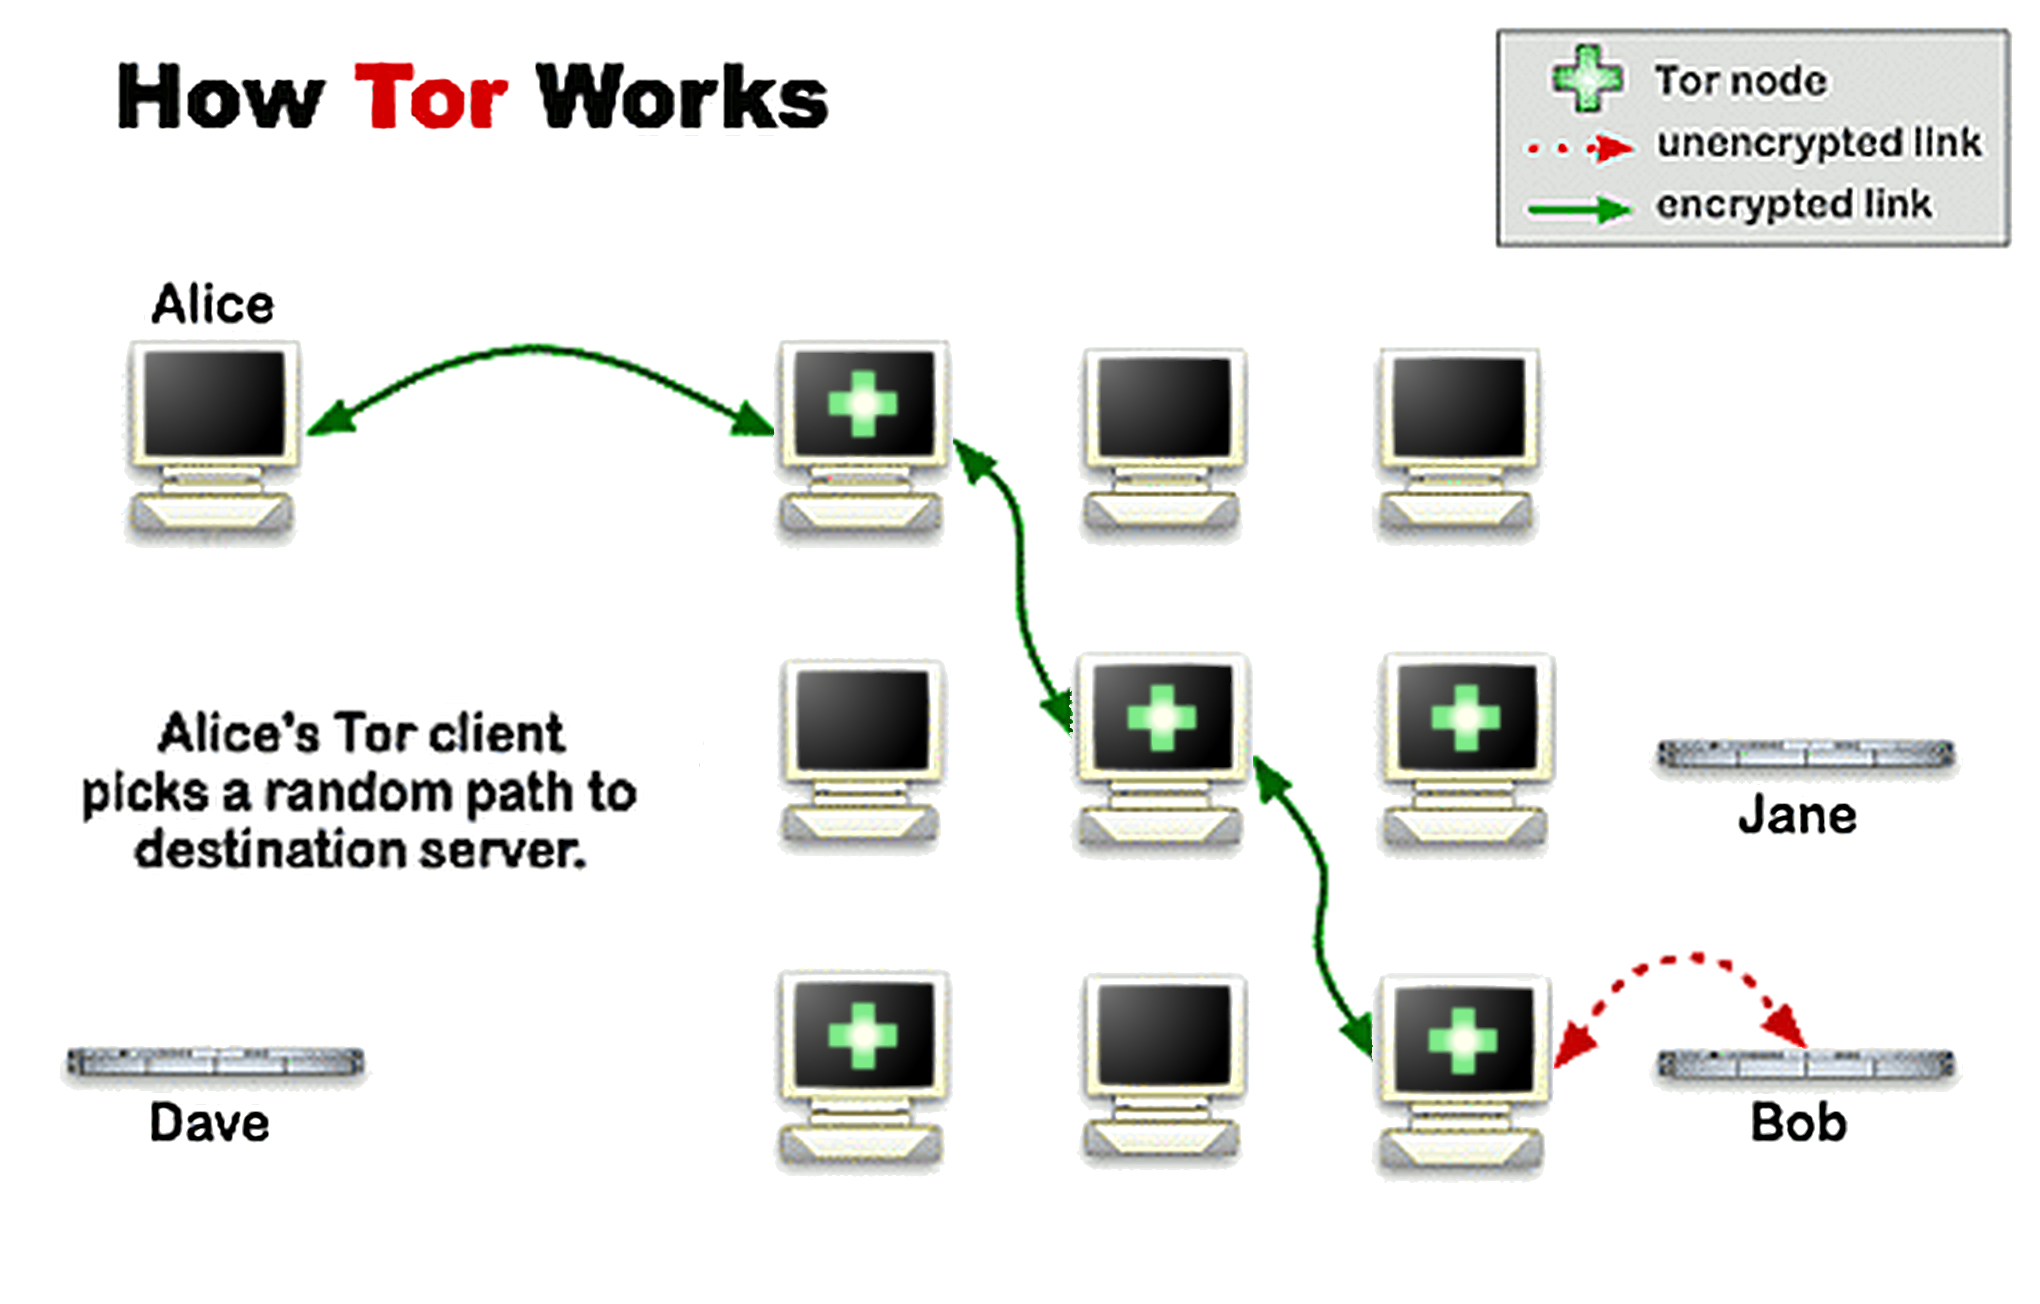
\includegraphics[width=\textwidth]{images/Tor/circuit-building-2-5.png}
		\caption{A circuit through the Tor network.}
		\label{fig:figure2}
	\end{minipage}
\end{figure}

\textit{Todo: the following paragraph is not a complete description of Tor's crypto. I don't describe the NTor routing protocol.}

The client first establishes a TLS connection with the first relay, $R_{1}$, using the relay's public key. The client then performs an ECDHE key exchange to negotiate $K_{1}$ which is then used to generate two symmetric session keys: a forward key $K_{1,F}$ and a backwards key $K_{1,B}$. $K_{1,F}$ is used to encrypt all communication from the client to $R_{1}$ and $K_{1,B}$ is used for all replies from $R_{1}$ to the client. These keys are used conjunction with the symmetric cipher suite negotiated during the TLS handshake, thus forming an encrypted tunnel with perfect forward secrecy. Once this one-hop circuit has been created, the client then sends $R_{1}$ the RELAY\_EXTEND command, the address of $R_{2}$, and the client's half of the Diffie-Hellman-Merkle protocol using $K_{1,F}$. $R_{1}$ performs a TLS handshake with $R_{2}$ and uses $R_{2}$'s public key to send this half of the handshake to $R_{2}$, who replies with his second half of the handshake and a hash of $K_{2}$. $R_{1}$ then forwards this to the client under $R_{1,B}$ with the RELAY\_EXTENDED command to notify the client. The client generates $K_{1,F}$ and $K_{1,B}$ from $K_{2}$, and repeats the process for $R_{3}$,\cite{ling2013protocol} as shown in Figure 3. The TCP/IP connections remain open, so the returned information travels back up the circuit to the end user.

Following the complete establishment of a circuit, the Tor client software then offers a Secure Sockets (SOCKS) interface on localhost which multiplexes any TCP traffic through Tor. At the application layer, this data is packed and padded into equally-sized Tor \textit{cells}, transmission units of 512 bytes. As each relay sees no more than one hop in the circuit, in theory neither an eavesdropper nor a compromised relay can link the connection's source, destination, and content. Tor further obfuscates user traffic by changing the circuit path every ten minutes,\cite{mccoy2008shining} as shown in Figure 4. A new circuit can also be requested manually by the user.

\begin{figure}[htbp]
	\centering
	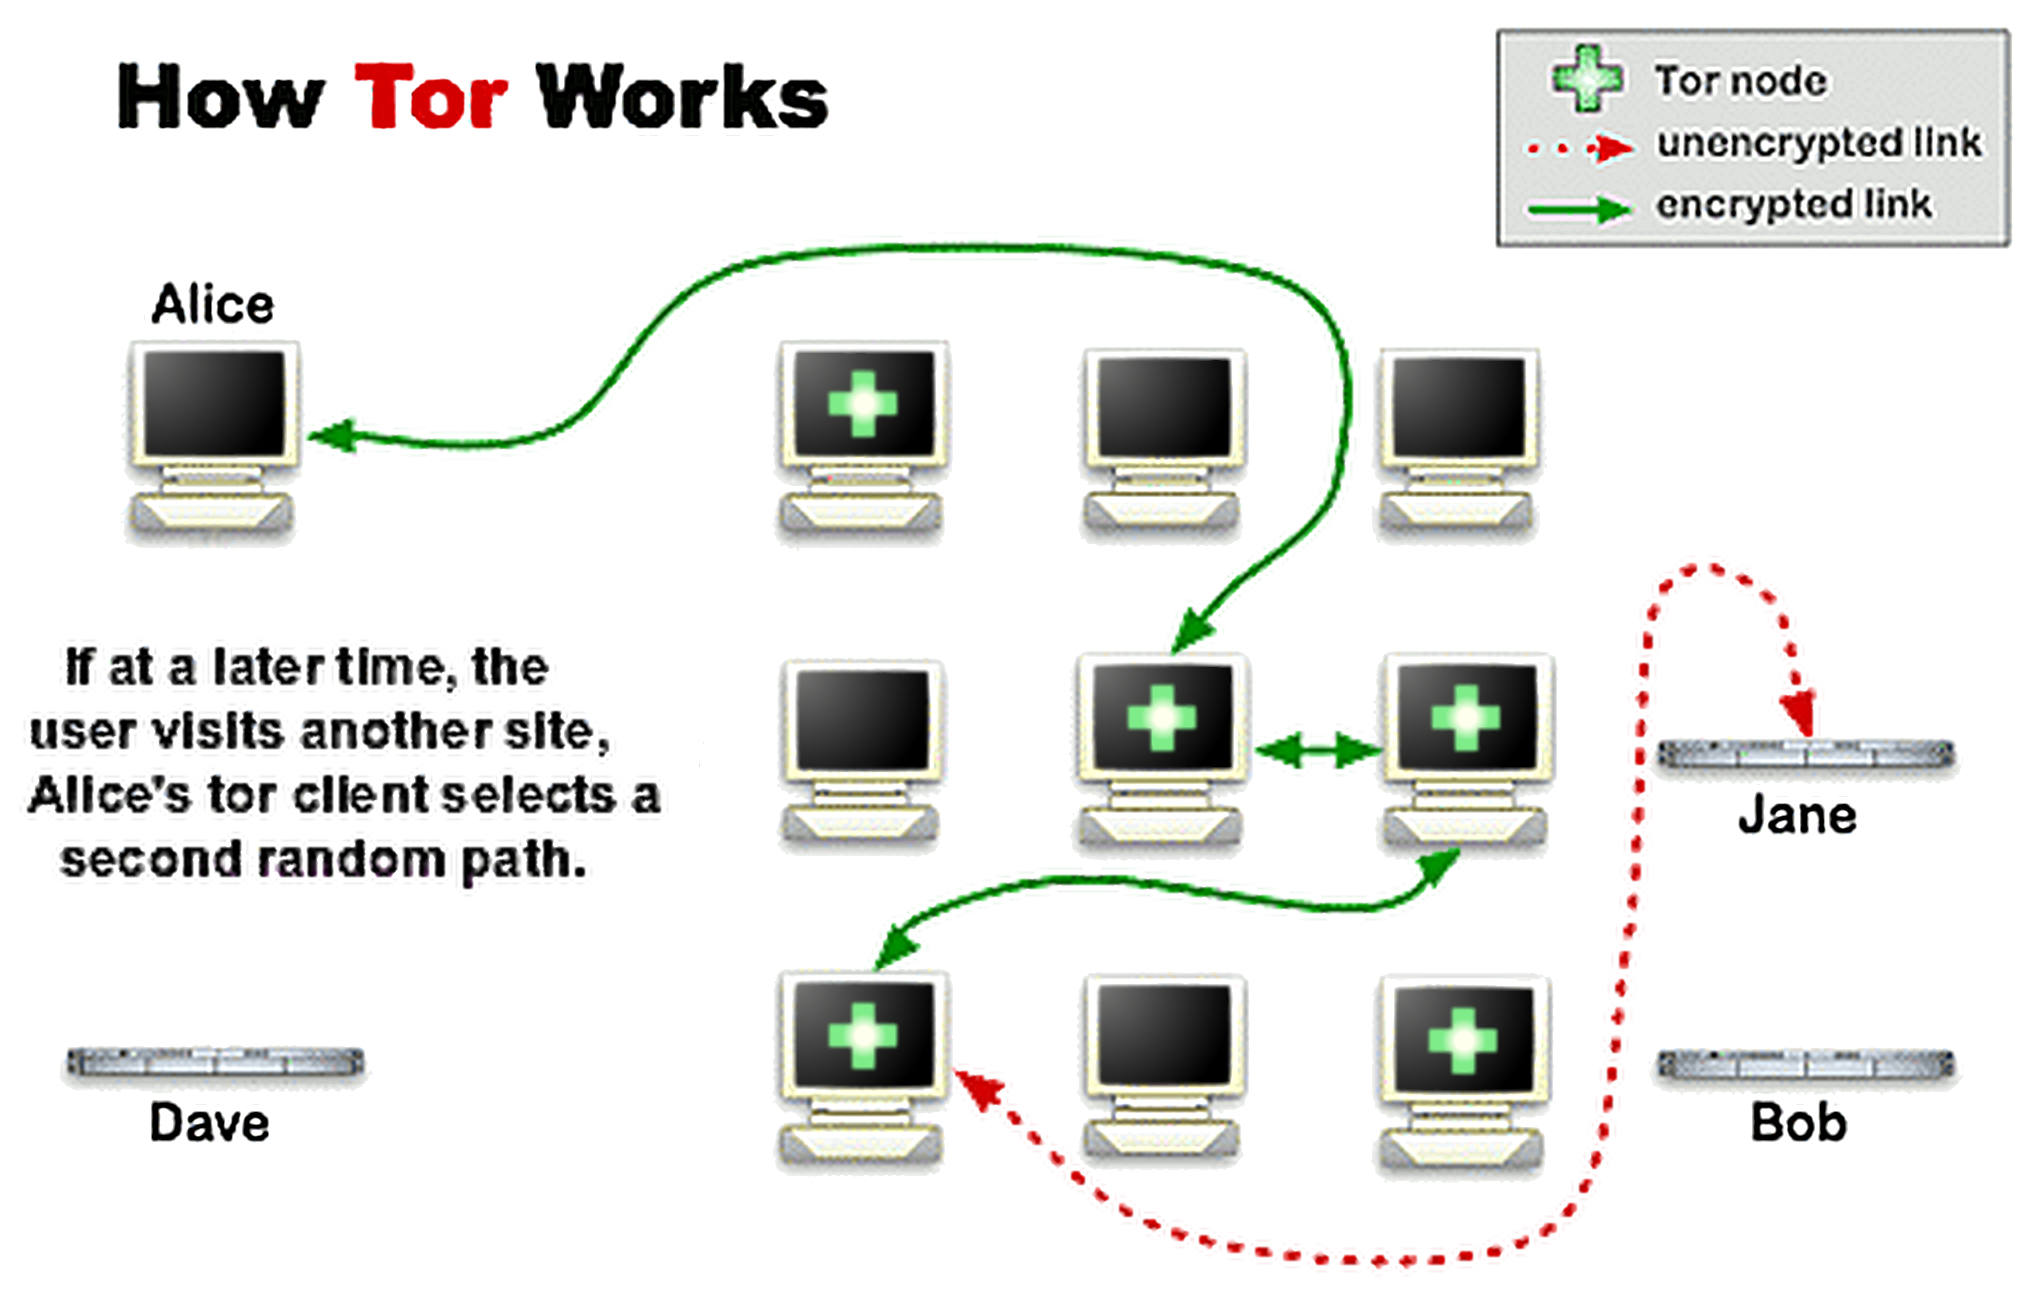
\includegraphics[width=0.6\textwidth]{images/Tor/circuit-change-1-4.png}
	\caption{A Tor circuit is changed periodically, creating a new user identity.}
\end{figure}

% Although a different guard node is used here, in practice the choice of entry point is preserved for extended periods of time.

Tor users typically use the Tor Browser, a custom build of Mozilla Firefox with a focus on security and privacy. The TBB anonymizes and provides privacy to the user in many ways. These include blocking all web scripts not explicitly whitelisted, forcing all traffic including DNS requests through the Tor SOCKS port, mimicking Firefox in Windows both with a user agent (regardless of the native platform) and SSL cipher suites, and reducing Javascript timer precision to avoid identification through clock skew. Furthermore, the TBB includes the Electronic Frontier Foundation's HTTPS Everywhere extension, which uses regular expressions to rewrite HTTP web requests into HTTPS for domains that are known to support HTTPS. If this is the case, an HTTPS connection will be established with the web server. If this happens, end-to-end encryption is complete and an outsider near the user would be faced with up to four layers of TLS encryption: $K_{1,F}(K_{2,F}(K_{3,F}(K_{server}(\textrm{client\ request}))))$ and likewise $K_{1,B}(K_{2,B}(K_{3,B}(K_{server}(\textrm{server\ reply}))))$ for the returning traffic, making traffic analysis very difficult.

\subsection{Hidden Services}

Although Tor's primary and most popular use is for secure access to the traditional Internet, since 2004 Tor also supports anonymous services, such as websites, marketplaces, or chatrooms. These are a part of the Dark Web and cannot be normally accessed outside the context of Tor. In contrast to Tor-anonymized web requests where the client is anonymous but the server is known, Tor hidden services provide bidirectional anonymity where both parties remain anonymous and never directly communicate with one another. This allows for a greater range of communication capabilities.\cite{nicolussi2011human}

Tor hidden services are known only by their public RSA key. Tor does not contain a DNS system for its websites; instead the domain names of hidden services are an 80-bit truncated SHA-1 hash of its public key, postpended by the .onion top-level domain (TLD). Once the hidden service is contacted and its public key obtained, this key can be checked against the requested domain to verify the authenticity of the service server. This process is analogous to SSL certificates in the clearnet, however Tor's authenticity check leaks no identifiable information about the anonymous server. If a client obtains the hash domain name of the hidden service through a backchannel and enters it into the Tor Browser, the hidden service lookup begins.

Preceding any client communication, the hidden server, Bob, first builds Tor circuits to several random relays and enables them to act as \textit{introduction points} by giving them its public key, $ B_{K} $. The server then uploads its public key and the fingerprint identity of these nodes to a distributed hashtable inside the Tor network, signing the result. When a client, Alice, requests contact with Bob, Alice's Tor software queries this hashtable, obtains $ B_{K} $ and Bob's introduction points, and builds a Tor circuit to one of them, $ ip_{1} $. Simultaneously, the client also builds a circuit to another relay, $ rp $, which she enables as a rendezvous point by telling it a one-time secret, $ sec $.

\begin{figure}[htdp]
	\begin{minipage}[b]{0.45\linewidth}
		\centering
		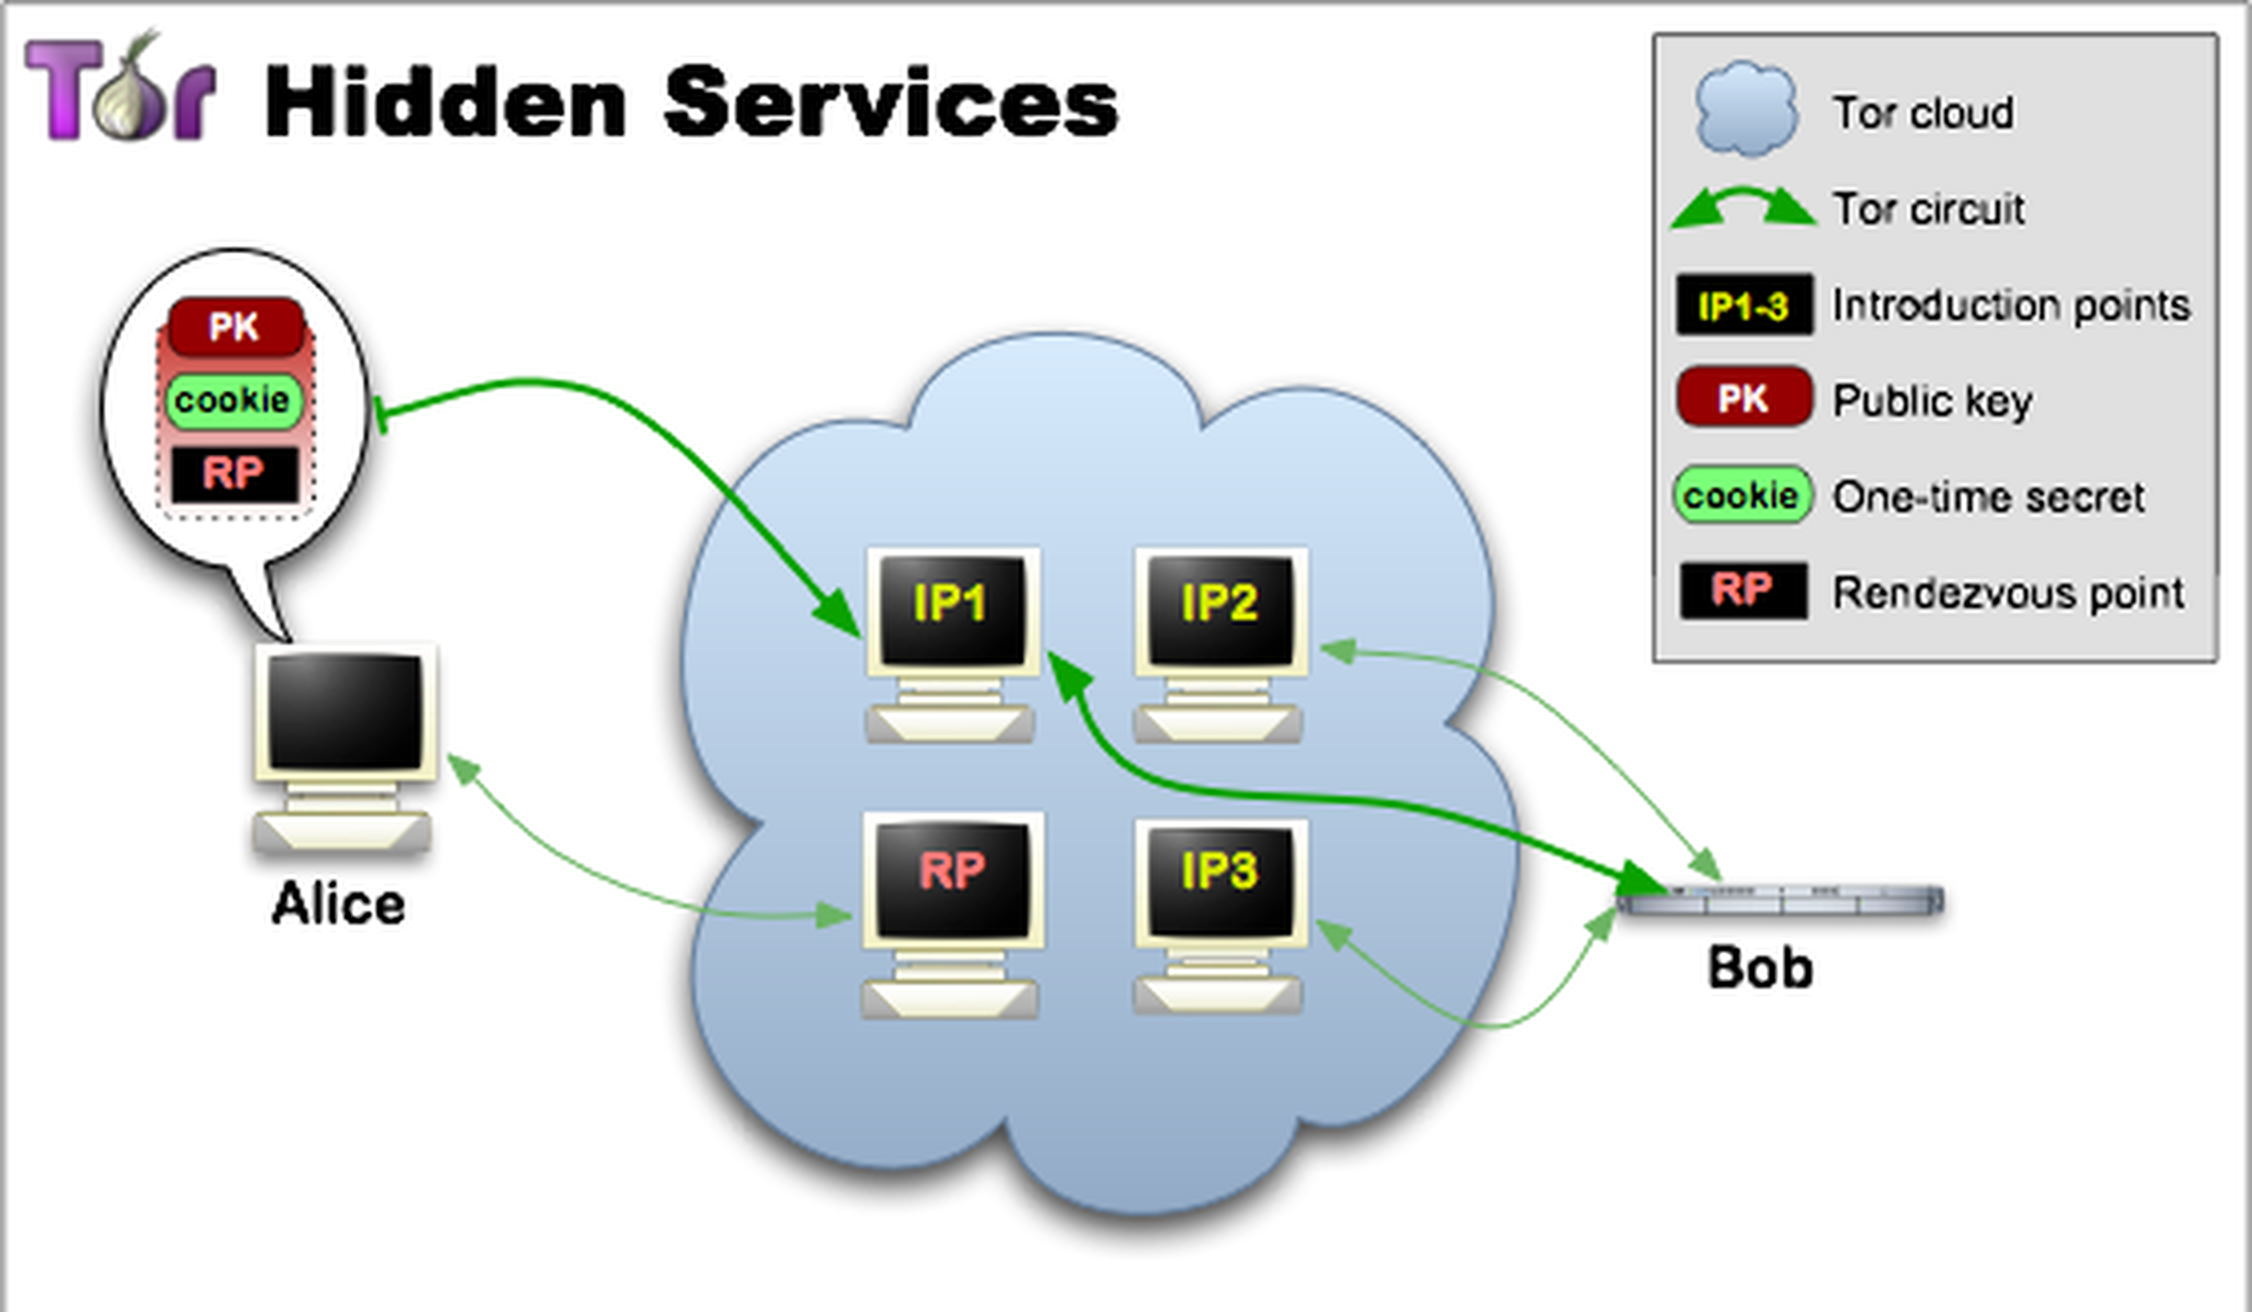
\includegraphics[width=\textwidth]{images/Tor/tor-hidden-service-4-higher.png}
		\caption{Alice uses the encrypted cookie to tell Bob to switch to $ rp $.}
	\end{minipage}
	\hspace{0.5cm}
	\begin{minipage}[b]{0.45\linewidth}
		\centering
		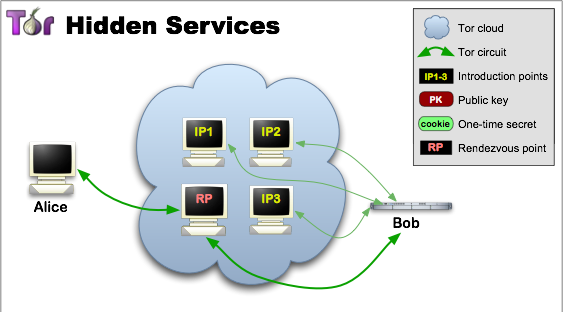
\includegraphics[width=\textwidth]{images/Tor/tor-hidden-service-6.png}
		\caption{Bidirectional communication between Alice and the hidden service.}
	\end{minipage}
\end{figure}

She then sends to $ ip_{1} $ a cookie encrypted with $ B_{K} $, containing $ rp $ and $ sec $. Bob decrypts this message, builds a circuit to $ rp $, and tells it $ sec $, enabling Alice and Bob to communicate. Their communication travels through six Tor nodes: three established by Alice and three by Bob, so both parties remain anonymous. From there traditional HTTP, FTP, SSH, or other protocols can be multiplexed over this new channel.

\section{Motivation}

The usability of hidden services is severely challenged by their non-intuitive 16-character base58-encoded domain names. To choose several prominent examples, 3g2upl4pq6kufc4m.onion is the address for the DuckDuckGo hidden service, 33y6fjyhs3phzfjj.onion is the Guardian's SecureDrop service for anonymous document submission, and blockchainbdgpzk.onion is the anonymized edition of blockchain.info. It is rarely clear what service a hidden server is providing by its domain name alone without relying on third-party directories for the correlation, directories which must be updated and reliably maintained constantly. These must be then distributed through backchannels such as /r/onions, the-hidden-wiki.com, or through a hidden service that is known in advance. It is a frequent topic of conversation inside Tor communities. It is clear that this problem limits the usability and popularity of Tor hidden services. Although there have been some workarounds that are partially successful, the issue remains unresolved. It is for these reasons that I propose EsgalDNS as a full solution.
